
\section{Appendix}

\subsection{Annotation Guidelines}
\label{sec: annotation guidelines}

\textbf{Guide for Dialogue Summarization Quality Evaluation}\\
Guidelines by: M. Gao and X. Wan. “DialSummEval: Revisiting Summarization Evaluation for Dialogues.” Alterations made for the present paper are preceded by ``Addition:''\\

\textbf{1. Instructions}

In this task you will evaluate the quality of summaries written for a dialogue from daily life.\\
To correctly solve this task, follow these steps:\\
1. Carefully read this dialogue, be aware of the information it contains.\\
2. Read the proposed summaries A-N (14 in total).\\
3. Rate each summary on a scale from 1(worst) to 5(best) by its consistency, relevance, fluency, coherence.\\

\textbf{2. Definitions}
\begin{enumerate}
    \item \textbf{Relevance (1-5)}: The rating measures how well the summary captures the key points of the dialogue. Consider whether all and only the important aspects are contained in the summary.
    \item \textbf{Consistency (1-5)}: The rating measures whether the facts in the summary are consistent with the facts in the dialogue. Consider whether the summary does reproduce all facts accurately and does not make up untrue information.
    \item \textbf{Fluency (1-5)}: The rating measures the quality of individual sentences, are they well-written and grammatically correct. Consider the quality of individual sentences.
    \item \textbf{Coherence (1-5)}: The rating measures the quality of all sentences collectively, to the fit together and sound naturally. Consider the quality of the summary as a whole. \textit{Addition: If the summary consists of one sentence, it receives a coherence score of 4}
\end{enumerate}


\textbf{3. Error Examples}

\textbf{Extrinsic Hallucination}: Content in summaries is not mentioned by dialogues. That is, the fact in the summary is neither supported nor contradicted by the source dialogue.\\

\textit{Example 1:}

Dialogue

 Luke: Hey sis, send me the pic of the parrot you painted yesterday?\\
 Gina: file\_photo\\
 Gina: If you want better quality I need to send you PDF file.\\
 Luke: It's ok. This parrot looks fantastic!!! I can't believe you've discovered your talent so late!\\
 Gina: Haha thanks? fil\_other Catch a PDF.\\
 Luke: Thanks!\\

Summary

Luke sent his sister , Gina , a photo of a parrot she painted yesterday .\\


\textit{Example 2:}

Dialogue

 Dave: Hey, is Nicky still at your place? Her phone is off\\
 Sam: She just left\\
 Dave: Thanks!\\
 
Summary

Nicky just left her phone at Dave ' s place .\\

\textbf{Wrong References}: Summaries contain information that is not faithful to
the original dialogue, and associate one’s actions/locations with a wrong speaker.\\

\textit{Example 1:}

Dialogue

Liam: will pick you up at 8\\
Liam: be ready\\
Kane: cool man\\
Liam: just don't get us late please\\

Summary

Liam will pick Liam up at 8 .\\

\textit{Example 2:}

Dialogue

 Ola: Hey running late\\
 Ola: I should be free by 8\\
 Kurt: Sure no prob, call me\\
 
Summary

Ola will be late. Kurt will call him by 8.\\

\textbf{Incorrect Reasoning:} Summaries reasoned relations in dialogues incorrectly,
thus came to wrong conclusions.\\

\textit{Example 1:}

Dialogue

 Sean: Hey, I won't be able to take the car to the carwash\\
 Sean: They want me to finish report first :(\\
 Alice: shoot, but it's crazily dirty\\
 Alice: Will we have tomorrow?\\
 Sean: file\_gif\\
 Sean: We can leave a bit earlier or get it washed somewhere on the road\\
 Alice: it might be  good idea, let's do it tomorrow then\\
 Sean: great!\\

Summary

Sean won't be able to take the car to the carwash tomorrow.\\

\textit{Example 2:}

Dialogue

 Sophie: When r u going to Poanań?\\
 Murphy: On Tuesday.\\
 Sophie: And you're coming back the same day?\\
 Murphy: Yes, in the afternoon, but I don't know the exact hour.\\

Summary

Murphy is going to Poanań on Tuesday and coming back the same day in the afternoon.\\


\textit{\textbf{Grammatical Error}}: The grammar of the sentence is so wrong that it becomes meaningless.\\
\textit{Example:} The Ebola vaccine accepted have already started.\\


\textbf{4. A potential scoring criterion}\\
Using consistency as an example\\
5 points: The facts in the summary are\textbf{ all} consistent with the facts in the dialogue.\\
4 points: \textbf{A small part} of the facts in the summary are not consistent with the facts in the dialogue.\\
3 points: \textbf{Some of} the facts in the summary are consistent with the facts in the dialogue, while some are not.\\
2 points: \textbf{Most of the facts} in the summary are not consistent with the facts in the dialogue.\\
1 point:\textbf{ None of the facts} in the summary are consistent with the facts in the dialogue.\\





\subsection{Annotation Tool}
\label{tool}


\begin{figure}[H]
    \centering
    %\textwidth
    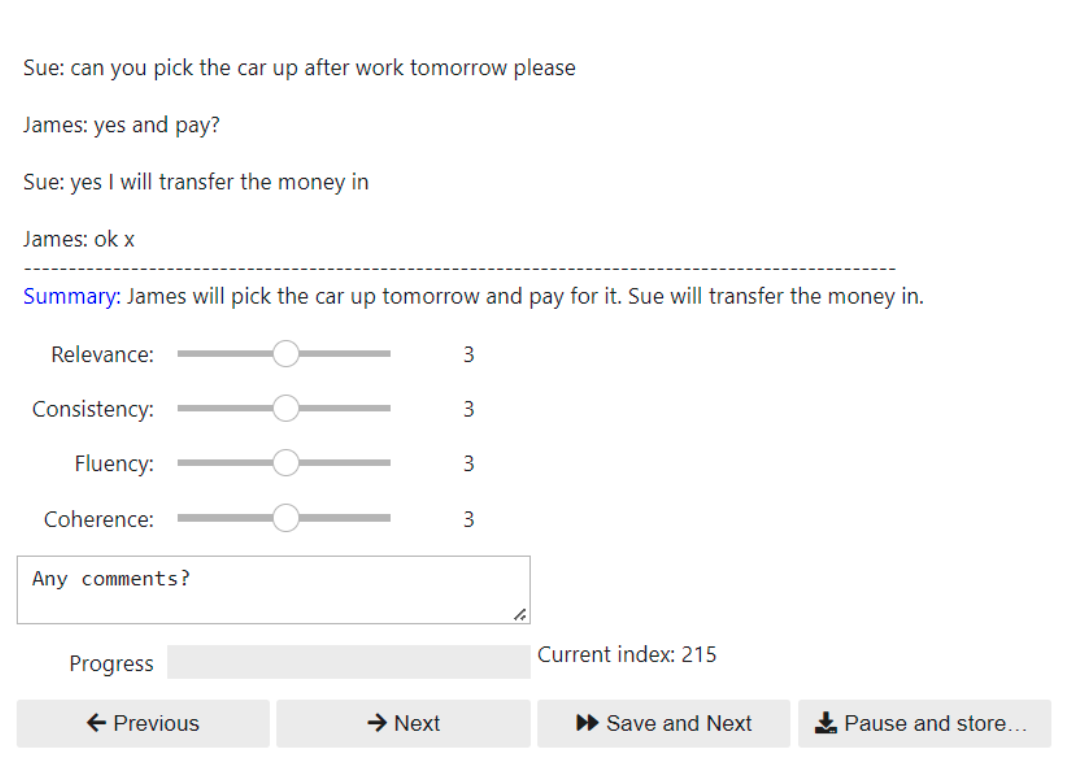
\includegraphics[width=140mm]{tool.png}
    \caption{Example of the annotation tool developed for the current reproduction study: The dialogue is presented at the top, followed by the current model or reference summary in blue. The sliding cursors can be adjusted for each dimension on a scale from 1 to 5. Inside the box below them, the annotators can write comments to facilitate decision tracking. Directly below that, the \textit{Current index} displays the number of data points annotated so far. The annotators can navigate the dataset by clicking on \textleftarrow \textit{Previous} and \textrightarrow \textit{Next}, but without saving the scores of the current summary. To achieve the latter they have to click on \textit{Save and Next}, while \textit{Pause and store} can be used for taking a break, while ensuring that their progress is saved.}
    \label{fig:tool}
\end{figure}


\subsection{Numerical differences}
\label{numeric}

\begin{table}
\centering
\resizebox{\linewidth}{!}{%
\begin{tabular}{l|cc|cc|cc|cc} 
\hline
                 & \multicolumn{2}{c|}{Coherence} & \multicolumn{2}{c|}{Consistency} & \multicolumn{2}{c|}{Fluency} & \multicolumn{2}{c}{Relevance}  \\ 
\hline
Metrics          & sys   & sum                    & sys   & sum                      & sys   & sum                  & sys   & sum                    \\ 
\hline
ROUGE-1          & 0.08  & 0.19                   & -0.04 & -0.08                    & 0.08  & 0.19                 & 0.33  & 0.12                   \\
ROUGE-2          & 0.05  & 0.14                   & -0.05 & -0.08                    & 0.06  & 0.14                 & 0.25  & 0.10                   \\
ROUGE-3          & 0.02  & 0.10                   & -0.05 & -0.07                    & 0.05  & 0.11                 & 0.20  & 0.07                   \\
ROUGE-4          & 0.01  & 0.08                   & -0.06 & -0.05                    & 0.04  & 0.09                 & 0.18  & 0.06                   \\
ROUGE-L          & 0.09  & 0.17                   & -0.04 & -0.07                    & 0.10  & 0.18                 & 0.33  & 0.14                   \\
BERTScore-p      & 0.27  & 0.29                   & -0.02 & -0.03                    & 0.28  & 0.27                 & 0.45  & 0.26                   \\
BERTScore-r      & 0.02  & 0.15                   & -0.05 & -0.10                    & 0.02  & 0.13                 & 0.22  & 0.04                   \\
BERTScore-f1     & 0.16  & 0.24                   & -0.04 & -0.07                    & 0.17  & 0.22                 & 0.36  & 0.17                   \\
MoverScore       & 0.07  & 0.17                   & -0.05 & -0.08                    & 0.09  & 0.16                 & 0.29  & 0.10                   \\
SMS              & 0.00  & 0.06                   & -0.06 & -0.06                    & 0.03  & 0.07                 & 0.16  & 0.05                   \\
BARTScore-s-h+   & -0.53 & -0.44                  & 0.03  & 0.00                     & -0.50 & -0.36                & -0.34 & -0.25                  \\
BARTScore-h      & 0.07  & 0.04                   & 0.01  & 0.03                     & 0.07  & 0.04                 & 0.14  & 0.08                   \\
BARTScore-h-r    & -0.02 & 0.15                   & -0.05 & -0.14                    & -0.03 & 0.13                 & 0.20  & -0.01                  \\
BARTScore-r-h    & 0.18  & 0.18                   & -0.02 & -0.02                    & 0.18  & 0.19                 & 0.43  & 0.21                   \\
BLANC-help+      & -0.47 & -0.35                  & -0.02 & -0.09                    & -0.51 & -0.35                & -0.49 & -0.39                  \\
BLANC-tune+      & -0.45 & -0.36                  & -0.02 & -0.08                    & -0.50 & -0.36                & -0.50 & -0.36                  \\
FEQA+            & 0.07  & 0.14                   & 0.05  & -0.01                    & 0.08  & 0.14                 & 0.38  & 0.12                   \\
QuestEval+       & -0.40 & -0.11                  & 0.04  & -0.09                    & -0.44 & -0.12                & -0.11 & -0.13                  \\
SummaQA-conf+    & -0.58 & -0.31                  & -0.01 & -0.06                    & -0.55 & -0.25                & -0.44 & -0.26                  \\
SummaQA-fscore+  & -0.48 & -0.21                  & -0.03 & -0.02                    & -0.53 & -0.18                & -0.46 & -0.22                  \\
PPL-             & 0.30  & 0.07                   & 0.01  & 0.05                     & 0.32  & 0.07                 & 0.08  & 0.13                   \\
CHRF             & 0.01  & 0.14                   & -0.05 & -0.10                    & 0.01  & 0.12                 & 0.21  & 0.03                   \\
BLEU-1           & 0.06  & 0.18                   & -0.05 & -0.09                    & 0.07  & 0.15                 & 0.21  & 0.05                   \\
BLEU-2           & 0.03  & 0.12                   & -0.06 & -0.08                    & 0.04  & 0.11                 & 0.17  & 0.05                   \\
BLEU-3           & 0.02  & 0.10                   & -0.06 & -0.07                    & 0.04  & 0.09                 & 0.15  & 0.05                   \\
BLEU-4           & 0.00  & 0.07                   & -0.06 & -0.06                    & 0.03  & 0.07                 & 0.13  & 0.04                   \\
METEOR           & 0.01  & 0.12                   & -0.06 & -0.09                    & 0.02  & 0.11                 & 0.19  & 0.05                   \\
EmbeddingAverage & 0.35  & 0.36                   & -0.05 & -0.11                    & 0.25  & 0.29                 & 0.44  & 0.12                   \\
VectorExtrema    & 0.09  & 0.21                   & -0.05 & -0.08                    & 0.10  & 0.18                 & 0.29  & 0.12                   \\
GreedyMatching   & 0.13  & 0.21                   & -0.05 & -0.11                    & 0.11  & 0.19                 & 0.29  & 0.07                   \\
FactCC+          & -0.54 & -0.41                  & -0.01 & 0.02                     & -0.50 & -0.32                & -0.49 & -0.23                  \\
DAE+             & -0.55 & -0.46                  & 0.01  & -0.02                    & -0.52 & -0.41                & -0.50 & -0.28                  \\
\hline
\end{tabular}

}\caption{Differences between the present paper and \citet{gao2022dialsummeval} for the correlation between the metrics and human evaluations, represented numerically}
\end{table}



\begin{table}
\centering
\resizebox{\linewidth}{!}{%
\begin{tabular}{lccccccc} 
\hline
Models       & Coherence & Consistency & Fluency & Relevance & R‐1 & R‐2 & R‐L  \\ 
\hline
reference    & 0.26      & 0.55        & 0.32    & 0.08      & 0   & 0   & 0    \\ 
\hline
LONGEST‐3    & -1.81     & 0.57        & -1.12   & -1.25     & 0   & 0   & 0    \\
LEAD‐3       & -1.95     & 0.84        & -1.10   & -1.02     & 0   & 0   & 0    \\
PGN          & -0.08     & 0.15        & -0.13   & -0.59     & 0   & 0   & 0    \\
Transformer  & -0.12     & -0.15       & -0.01   & -0.20     & 0   & 0   & 0    \\
BART         & 0.06      & 0.62        & 0.32    & -0.14     & 0   & 0   & 0    \\
PEGASUS      & -0.06     & 0.70        & 0.31    & -0.21     & 0   & 0   & 0    \\
UniLM        & -0.01     & 0.51        & 0.20    & -0.23     & 0   & 0   & 0    \\
CODS         & 0.10      & 0.64        & 0.34    & -0.11     & 0   & 0   & 0    \\
ConvoSumm    & 0.12      & 0.74        & 0.34    & -0.06     & 0   & 0   & 0    \\
MV‐BART      & 0.43      & 0.51        & 0.33    & 0.01      & 0   & 0   & 0    \\
PLM‐BART     & 0.27      & 0.62        & 0.25    & -0.01     & 0   & 0   & 0    \\
Ctrl‐DiaSumm & 0.41      & 0.51        & 0.31    & -0.01     & 0   & 0   & 0    \\
S‐BART       & 0.29      & 0.57        & 0.41    & -0.12     & 0   & 0   & 0    \\
\hline
\end{tabular}
}\caption{Numerical difference between average human rating between \citet{gao2022dialsummeval} and the present paper}
\end{table}
